% This program can be redistributed and/or modified under the terms
% of the GNU Public License, version 3.
%
% Seth Brown, Ph.D.
% sethbrown@drbunsen.org
%
% Compiled with XeLaTeX
% Dependencies:
%   Fontin Sans font (http://www.exljbris.com/fontinsans.html)
%
\documentclass{beamer}

\usepackage{graphicx} % graphics
\usepackage{epsfig} % eps graphics
\usepackage{hyperref} % urls
\usepackage{booktabs, caption} % table styling
\usepackage{subfig}

\definecolor{myblue}{HTML}{D4DEFF}
\definecolor{redcell}{HTML}{FFE8E8}
\definecolor{greencell}{HTML}{E8FFEB}
\definecolor{yellowcell}{HTML}{FFFDE8}
\newcommand{\vomega}{\vec{\omega}}
\newcommand{\x}{\mathbf{x}}
\newcommand{\cs}{C_{\phi}(\eta)}
\newcommand{\csinv}{C_{\phi}(1/\eta)}
\newcommand{\ce}{C_{\mathbf{E}}(\eta)}
\newcommand{\gl}[1]{\texttt{\nolinkurl{#1}}}
\newcommand\mycolor[1]{#1}
% suppress navigation bar
\beamertemplatenavigationsymbolsempty

\mode<presentation>
{
  \usetheme{bunsen}
  \setbeamercovered{transparent}
  \setbeamertemplate{items}[circle]
}

% set fonts
\usepackage{fontspec}
\setsansfont{Fontin Regular}
\setbeamerfont{frametitle}{size=\LARGE,series=\bfseries}

% color definitions
\usepackage{color}
\definecolor{uipoppy}{RGB}{153, 0, 0}
\definecolor{uipaleblue}{RGB}{153,153,153}
\definecolor{uiblack}{RGB}{0, 0, 0}

% caption styling
\DeclareCaptionFont{uiblack}{\color{uiblack}}
\DeclareCaptionFont{uipoppy}{\color{uipoppy}}
\captionsetup{labelfont={uipoppy},textfont=uiblack}

% see the macros.tex file for definitions
% This program can be redistributed and/or modified under the terms
% of the GNU Public License, version 3.

% adds reference to bottom right of corner of a slide
\usepackage[absolute,overlay]{textpos} % text references in slide corners
\newcommand\textref[1]{%
  \begin{textblock*}{\paperwidth}(0pt,0.99\textheight)
  \raggedleft \tiny{\emph{#1}}\hspace{.5em}
  \end{textblock*}}

% for drawing circles around numbers
% ex. \circled{1} Add some text here.
\usepackage{tikz}
\newcommand*\circled[1]{\tikz[baseline=(char.base)]{
            \node[shape=circle,draw,inner sep=2pt] (char) {#1};}}


% title slide definition
\title[Real-time Rendering of Translucent Materials]{Real-time Rendering of Translucent Materials with Directional Subsurface Scattering}
\author{Alessandro Dal Corso}
\institute[Università degli studi di Padova]
{
Laurea Magistrale in Ingegneria Informatica \\
M.Sc. in Digital Media Engineering \\
T.I.M.E. Double Degree Program\\*[2em] 
Relatore: Emanuele Menegatti\\
Correlatore: Jeppe Revall Frisvad
}

\date{7 Luglio 2014}

%--------------------------------------------------------------------
%                           Introduction
%--------------------------------------------------------------------

\begin{document}

\section{Introduction}
\setbeamertemplate{background}
{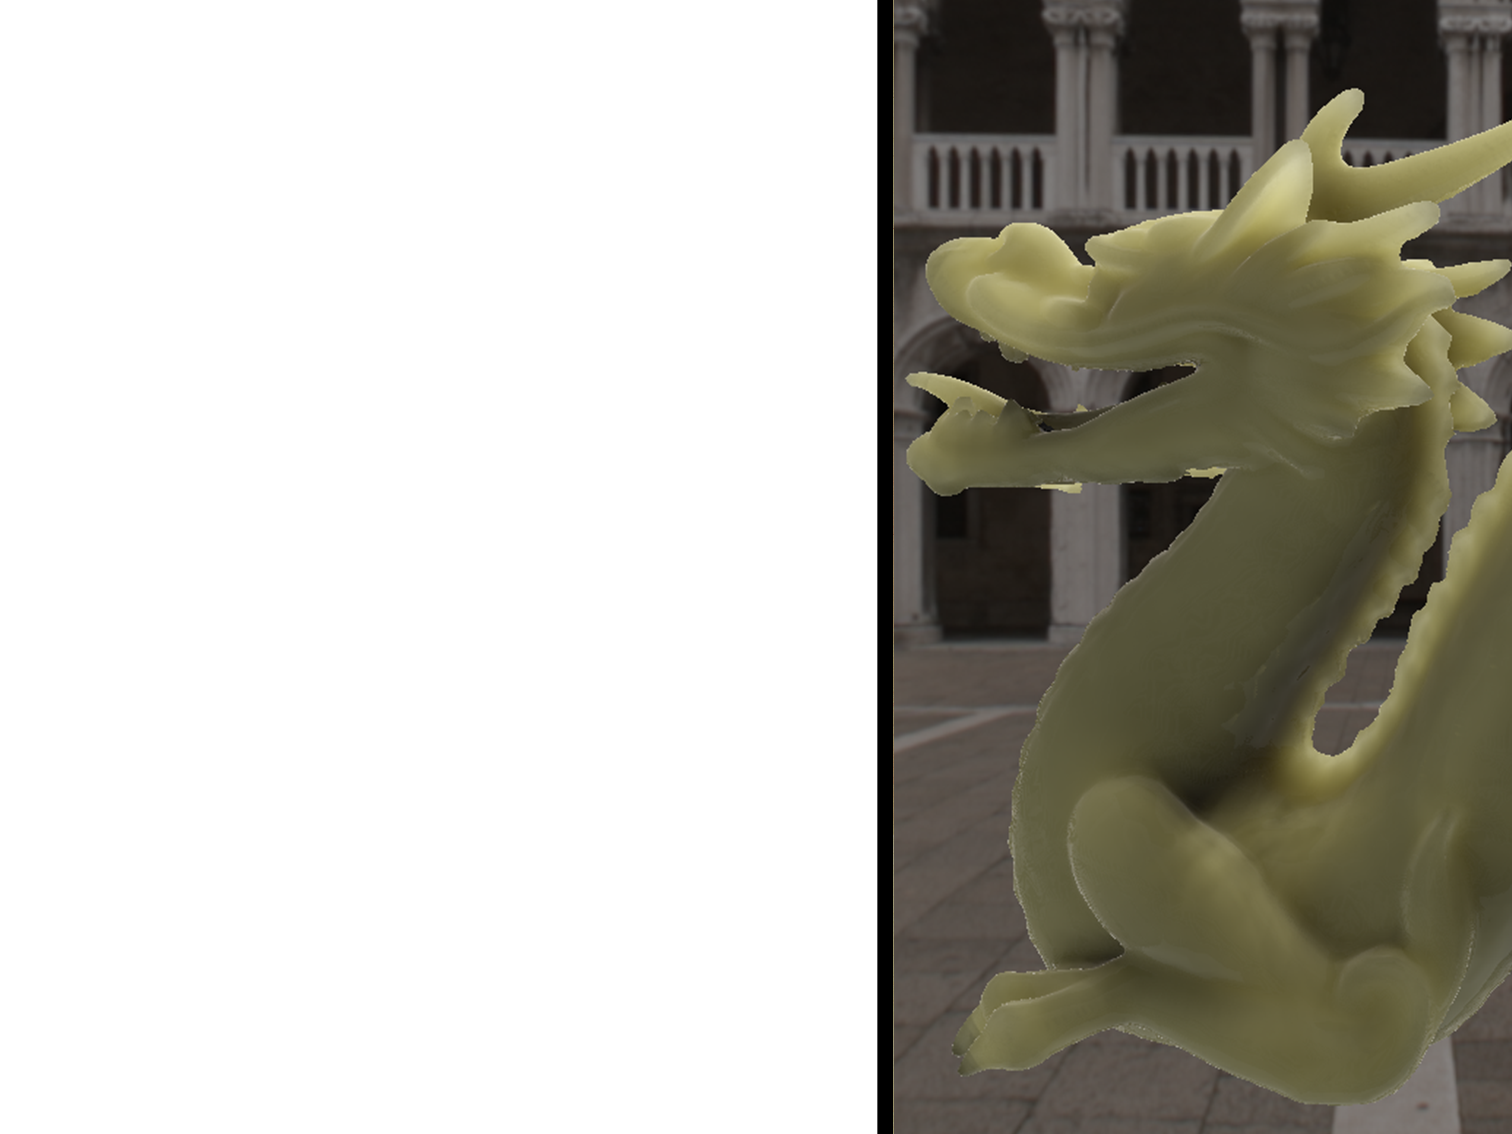
\includegraphics[width=\paperwidth,height=\paperheight]{frontpage_bg}}
\setbeamertemplate{footline}[default]

\begin{frame}
\vspace{1cm}
\begin{columns}
\column{2.75in}
  \titlepage
  \vspace{10cm}
\column{2.0in}
\end{columns}
\end{frame}

%-------------------------------------------------------------------
%                          Section 1
%-------------------------------------------------------------------
%
% Set the background for the rest of the slides.
% Insert infoline

\setbeamertemplate{background}
 {
\includegraphics[width=\paperwidth,height=\paperheight]{slide_bg}}
\setbeamertemplate{footline}[bunsentheme]

\section{Alessandro Dal Corso}
\begin{frame}
    \frametitle{Introduzione}
\begin{columns}[t]
    \begin{column}{0.55\textwidth}
      \centering
			\begin{itemize}
				\item Rendering di materiali traslucidi, come frutta, marmo, pelle
				\item Materiali con alto scattering sottosuperficiale
				\item Rendering interattivo ($>$ 10 FPS) 
				\item Applicazioni: computer games e visualizzazione digitale
			\end{itemize}
		\vspace{0.5cm}
		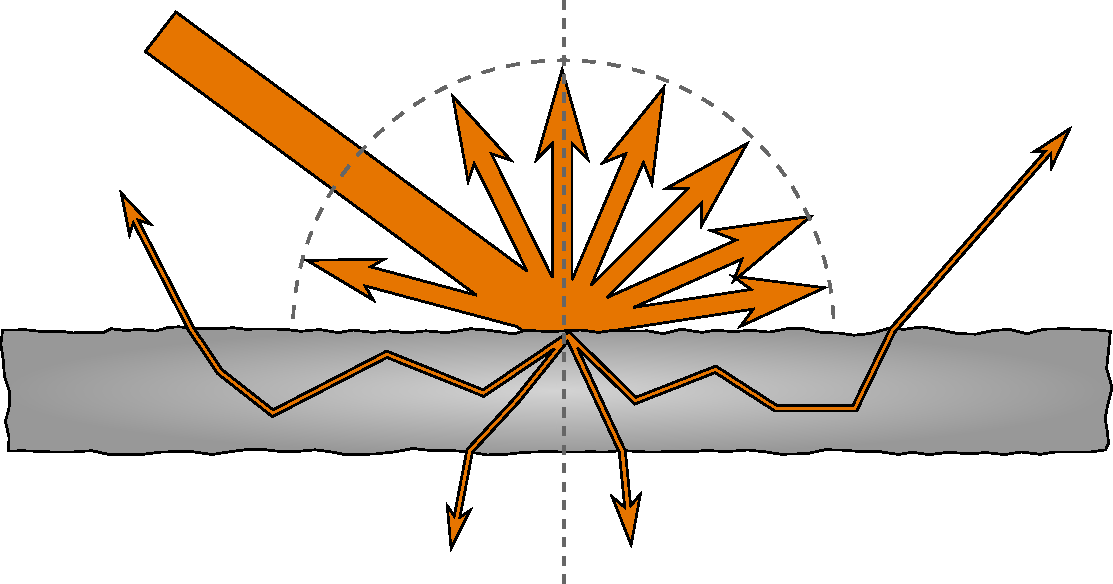
\includegraphics[width=0.5\paperwidth]{diagram}	
    \end{column}
    \begin{column}{0.45\textwidth}
		\vspace{0.0cm}
		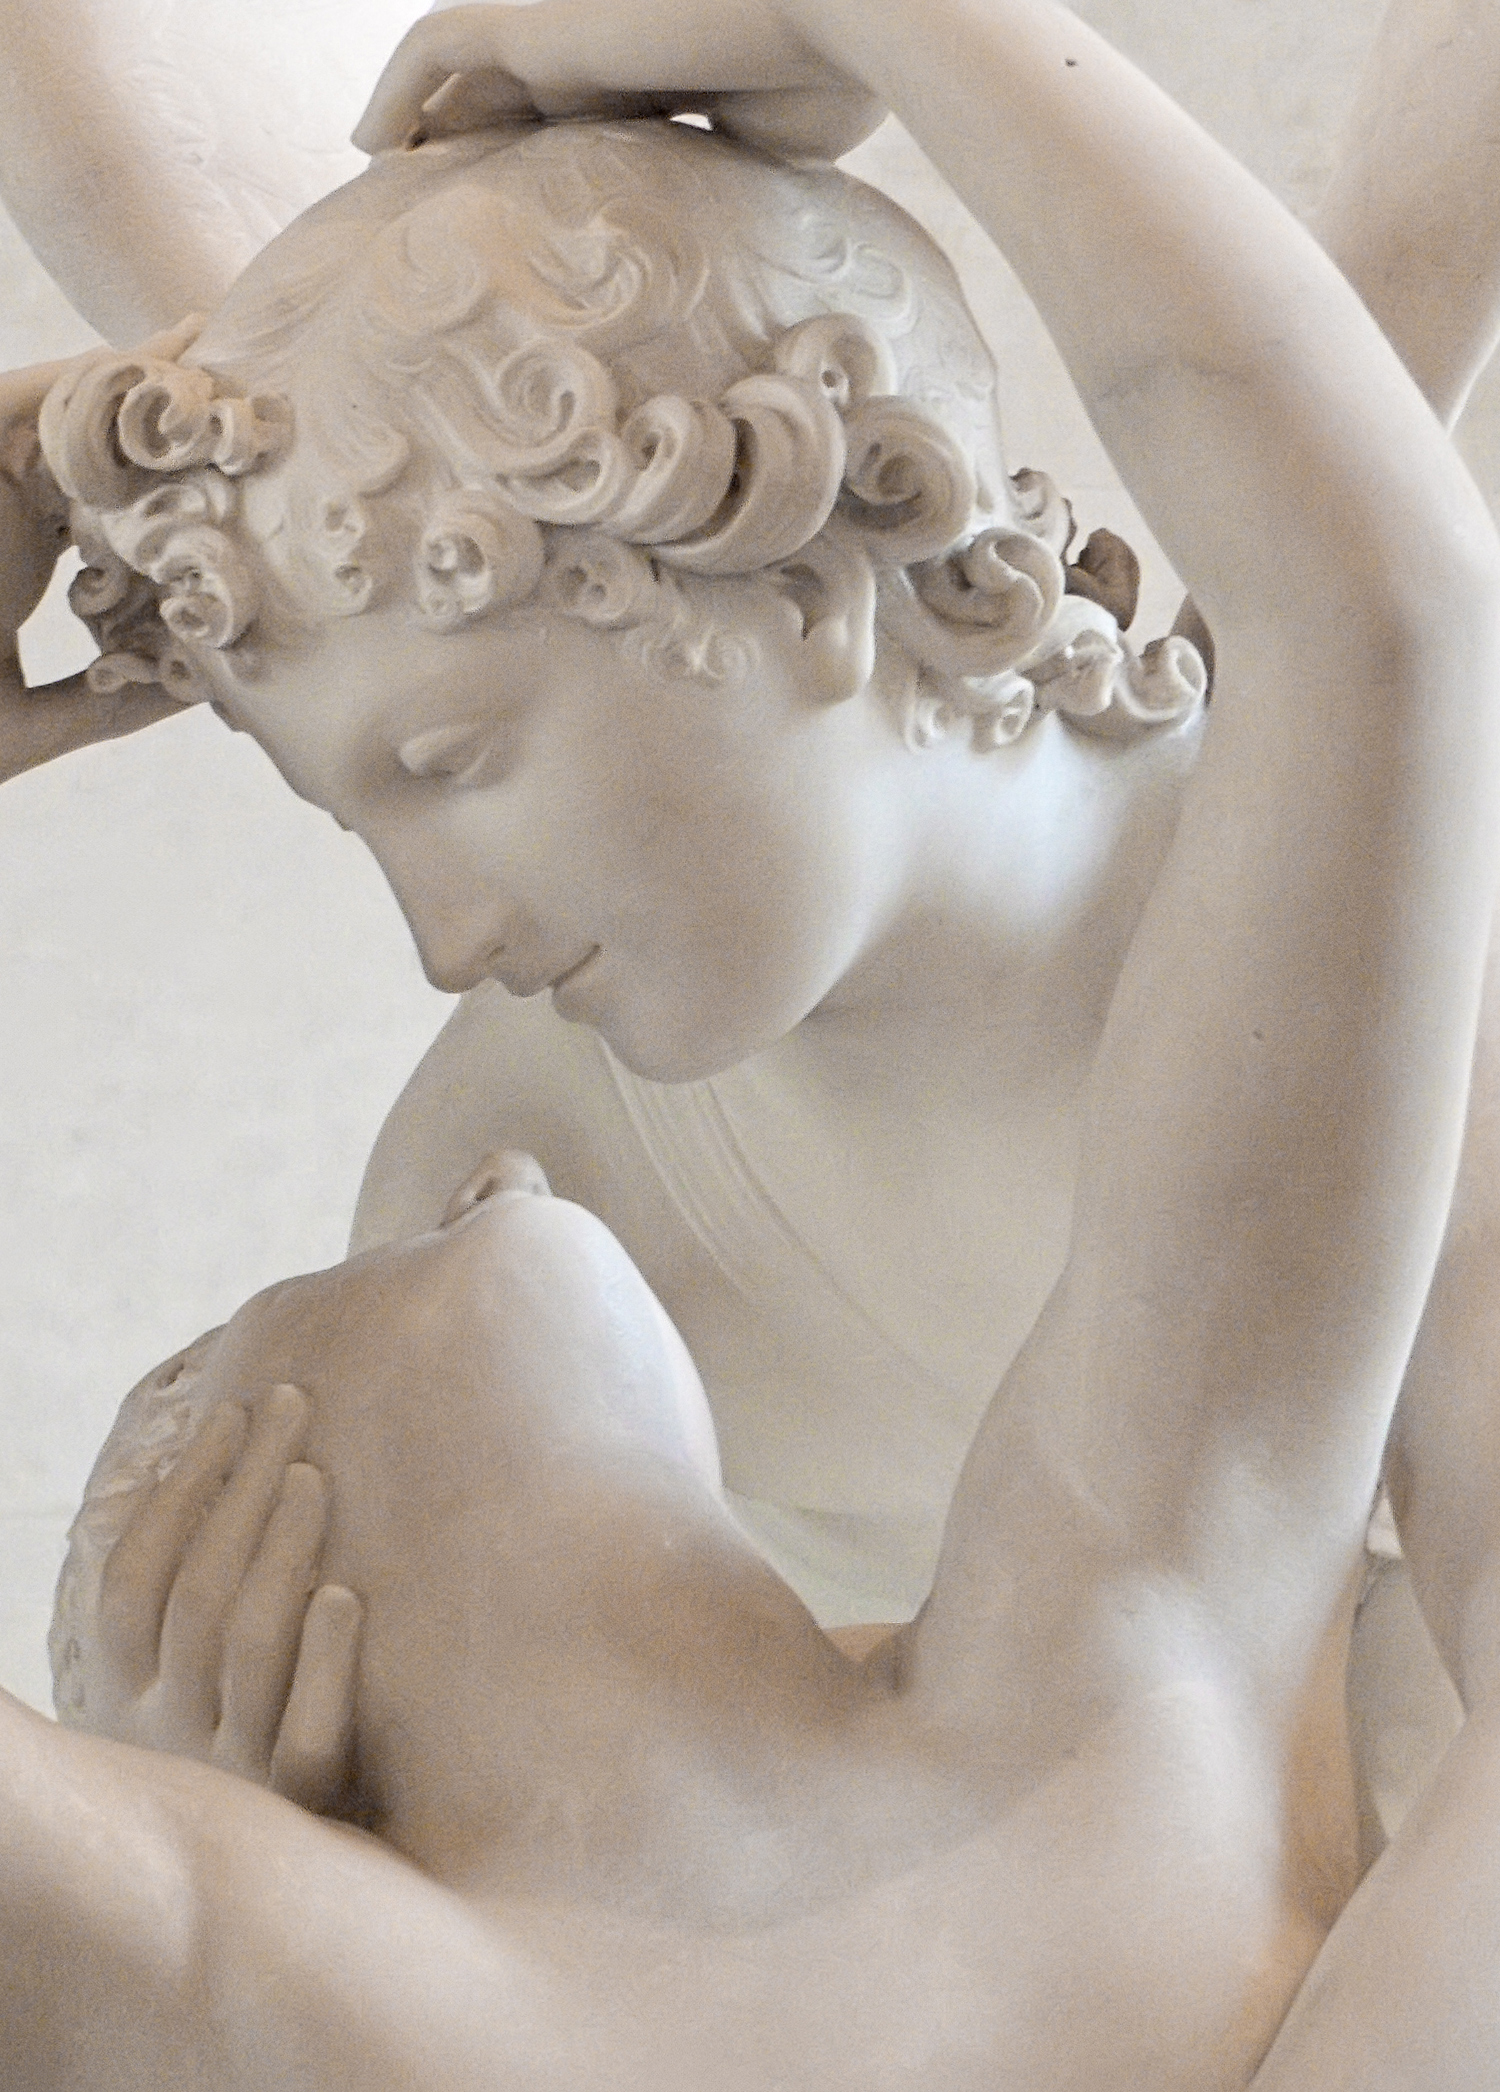
\includegraphics[width=0.5\paperwidth]{marble}
    \end{column}
​  \end{columns}
\end{frame}

\begin{frame}
    \frametitle{Light transport}
				\vspace{0.5cm}

\begin{columns}
    \begin{column}{0.5\textwidth}
			\begin{itemize}
				\item Definiamo una quantità fisica per descrivere la luce, detta \emph{radianza}:
			  $$L(\vomega) = \frac{d^2 \Phi}{d\omega dA \cos \theta}$$
			\end{itemize}
    \end{column}
    \begin{column}{0.5\textwidth}
		\centering
		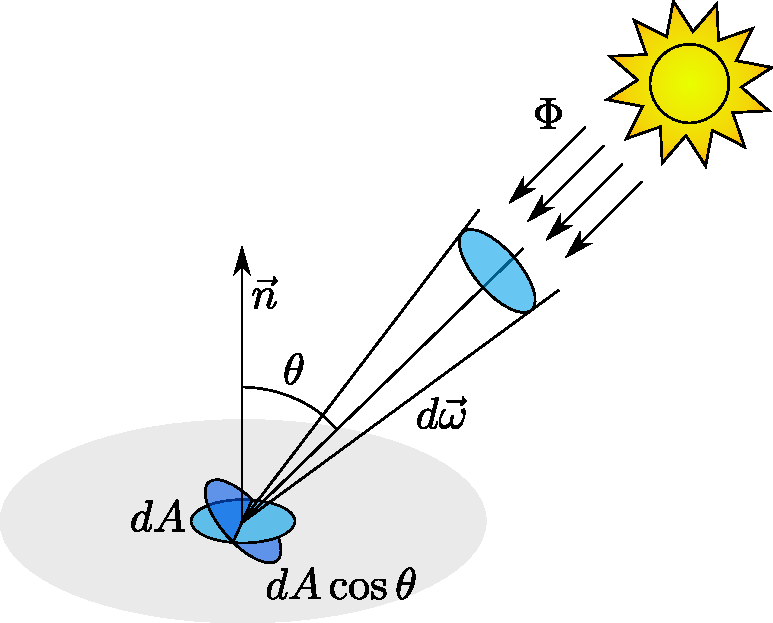
\includegraphics[width=0.7\textwidth]{radiance}
    \end{column}
​  \end{columns}
\vspace{0.3cm}
\begin{columns}
    \begin{column}{0.4\textwidth}
      \centering
		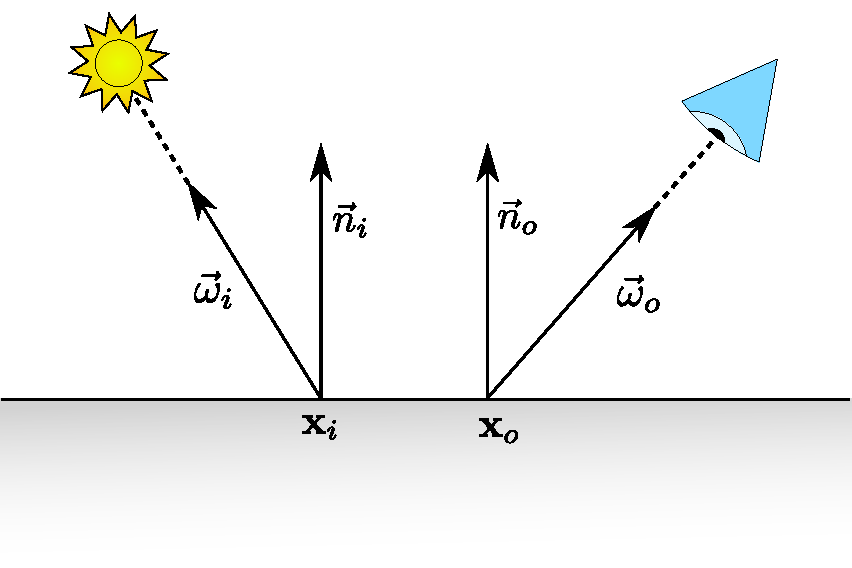
\includegraphics[width=\textwidth]{bssrdf}
				\end{column}
    \begin{column}{0.6\textwidth}
				\begin{itemize}
				\item Avendo due punti su una superficie, definiamo il BSSRDF come:
$$
S(\x_i, \vomega_i, \x_o, \vomega_o) = \frac{d L_o(\x_o,\vomega_o)}{L_i(\x_i,\vomega_i) \cos \theta_i d\vomega_i d A_i}  
$$			
				Che collega il flusso entrante con la radianza uscente.
\end{itemize}

    \end{column}
​  \end{columns}

\end{frame}

\begin{frame}
    \frametitle{The rendering equation}
			\begin{itemize}
				\item Dalla definizione di BSSRDF ottieniamo la cosiddetta \emph{rendering equation} [Jensen et al., 2001]:
				$$L_o(\x_o,\vomega_o) = L_e(\x_i,\vomega_i) + \int_A \int_{2\pi} S(\x_i, \vomega_i, \x_o, \vomega_o) L_i(\x_i,\vomega_i) (\vec{n} \cdot \vomega_i) d\vomega_i d A_i$$
				\item Ci sono vari BSSRDF in letteratura [Jensen et al., 2001; d'Eon et al., 2011; Frisvad et al., 2014]
			\end{itemize}
\end{frame}

\begin{frame}
    \frametitle{BSSRDF Direzionale}
		\vspace{0.3cm}
			\begin{itemize}
				\item {[}Frisvad et al, 2014{]} hanno definito un nuovo BSSRDF che tiene conto della direzione della luce incidente.
				\item L'effetto di scattering viene modellato come due sorgenti, una \emph{reale} e una \emph{virtuale}. \\
				\centering
				\vspace{0.2cm}
				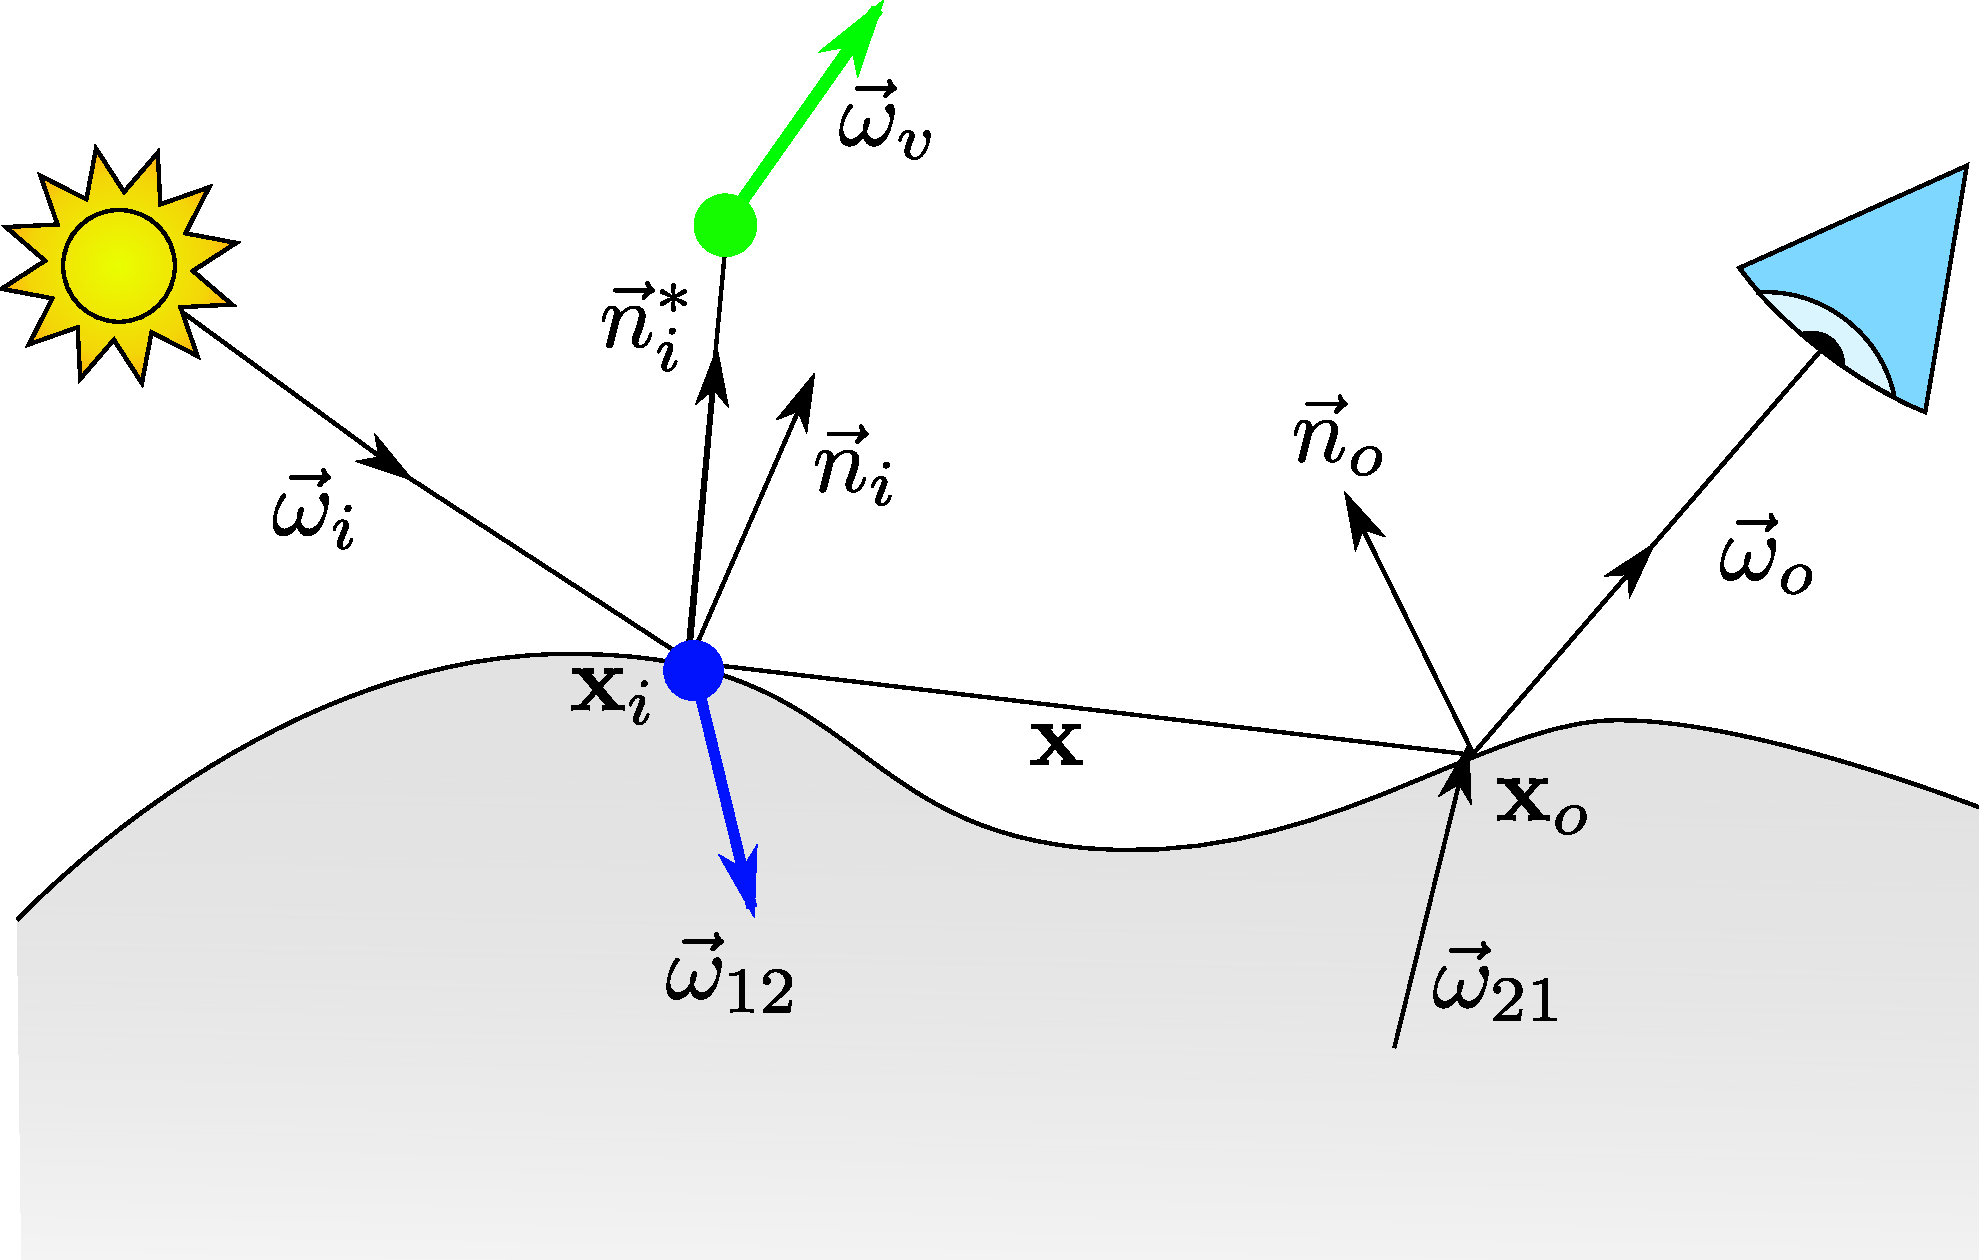
\includegraphics[width=0.55\textwidth]{jeppe}
			\end{itemize}
			$$
			S_d(\x_i, \vomega_i, \x_o) = S'_d(\x_o - \x_i, \vomega_{12}, d_r) - S'_d(\x_o - \x_v, \vomega_{v}, d_v)
			$$
\end{frame}

\begin{frame}
    \frametitle{Metodo}
			\begin{itemize}
			\item Gli effetti di scattering hanno un range limitato, che dipende dalle proprietà ottiche del materiale.
			\item Creiamo un disco di campionamento di area $A_c$.
			\item Approssimiamo la rendering equation (per luci direzionali):
				\vspace{-0.3cm}
				$$
				L_o(\x_o,\vomega_o) = L_d \frac{A_c}{N} \sum_{i = 1}^N S(\x_i, \vomega_l, \x_o, \vomega_o)  e^{\sigma_{tr} r_i}
				$$
				\vspace{-0.6cm}
				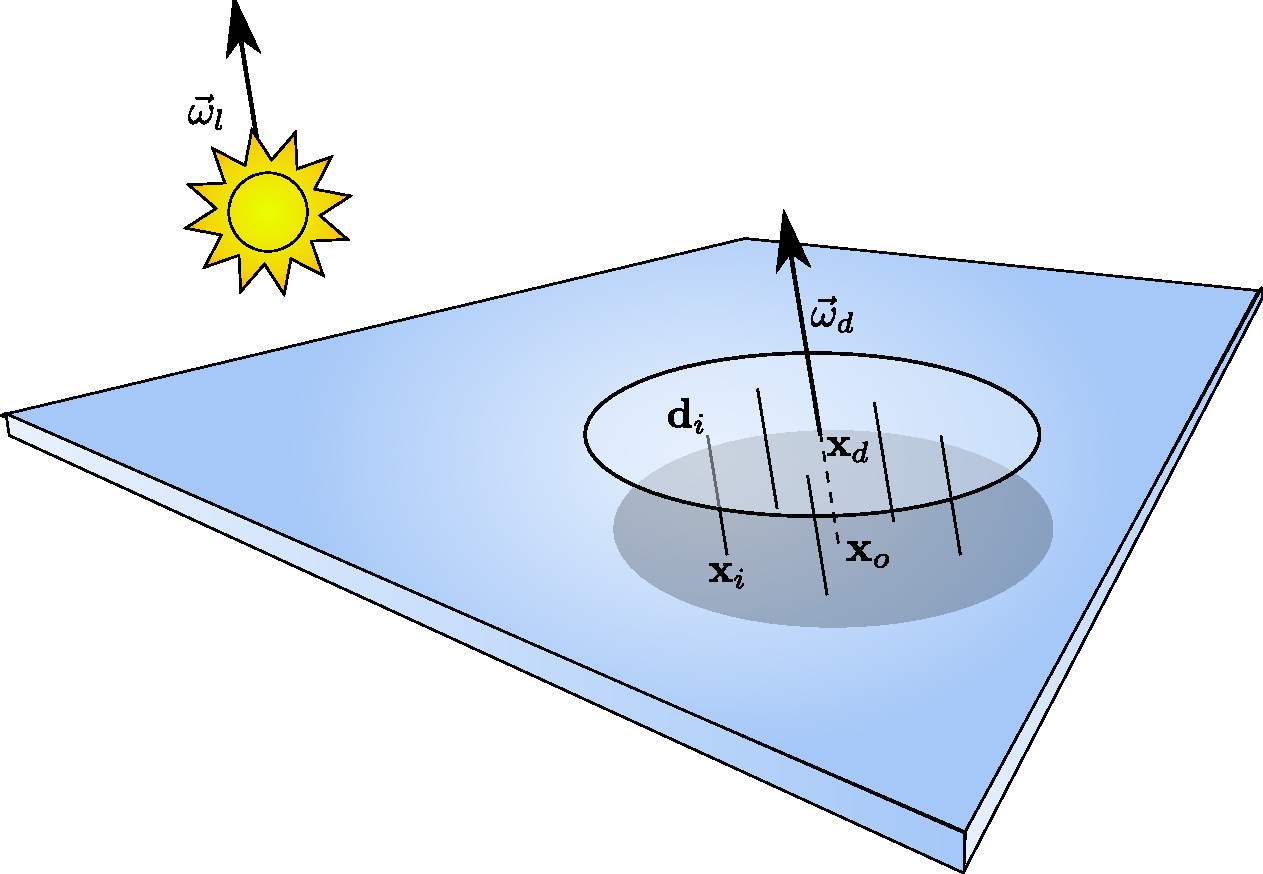
\includegraphics[width=0.4\textwidth]{disk_setup.pdf} \hspace{1cm}	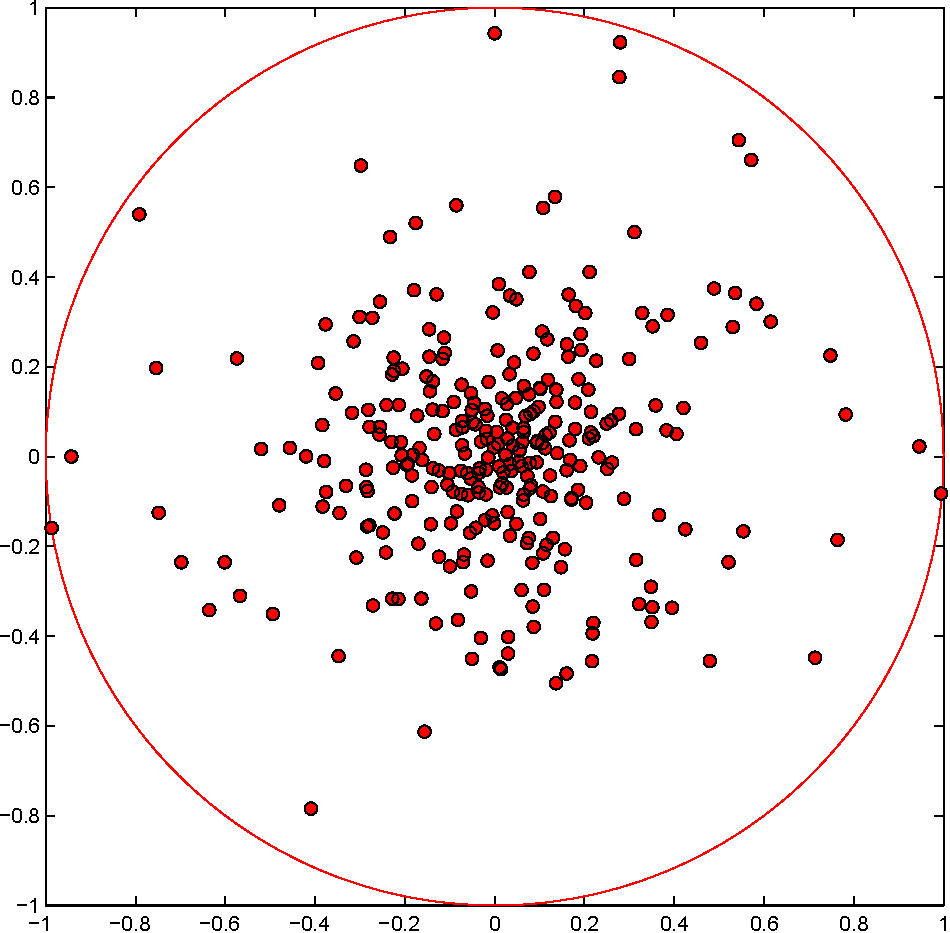
\includegraphics[width=0.3\textwidth]{halton_exp.pdf}
			\end{itemize}
\end{frame}

\begin{frame}
    \frametitle{Implementazione}
			\begin{itemize}
			\item Abbiamo implementato il nostro metodo su hardware GPU, usando OpenGL 4.3 (2012) e C++.
			\item Otteniamo il risultato finale in tre passi:
			\begin{itemize}
				\item[1] Rendering dell'oggetto dal punto di vista della luce
				\item[2] Rendering dell'oggetto da camere direzionali e accumulo del risultato
				\item[3] Ricostruzione del risultato. 
			\end{itemize}
			\end{itemize}
			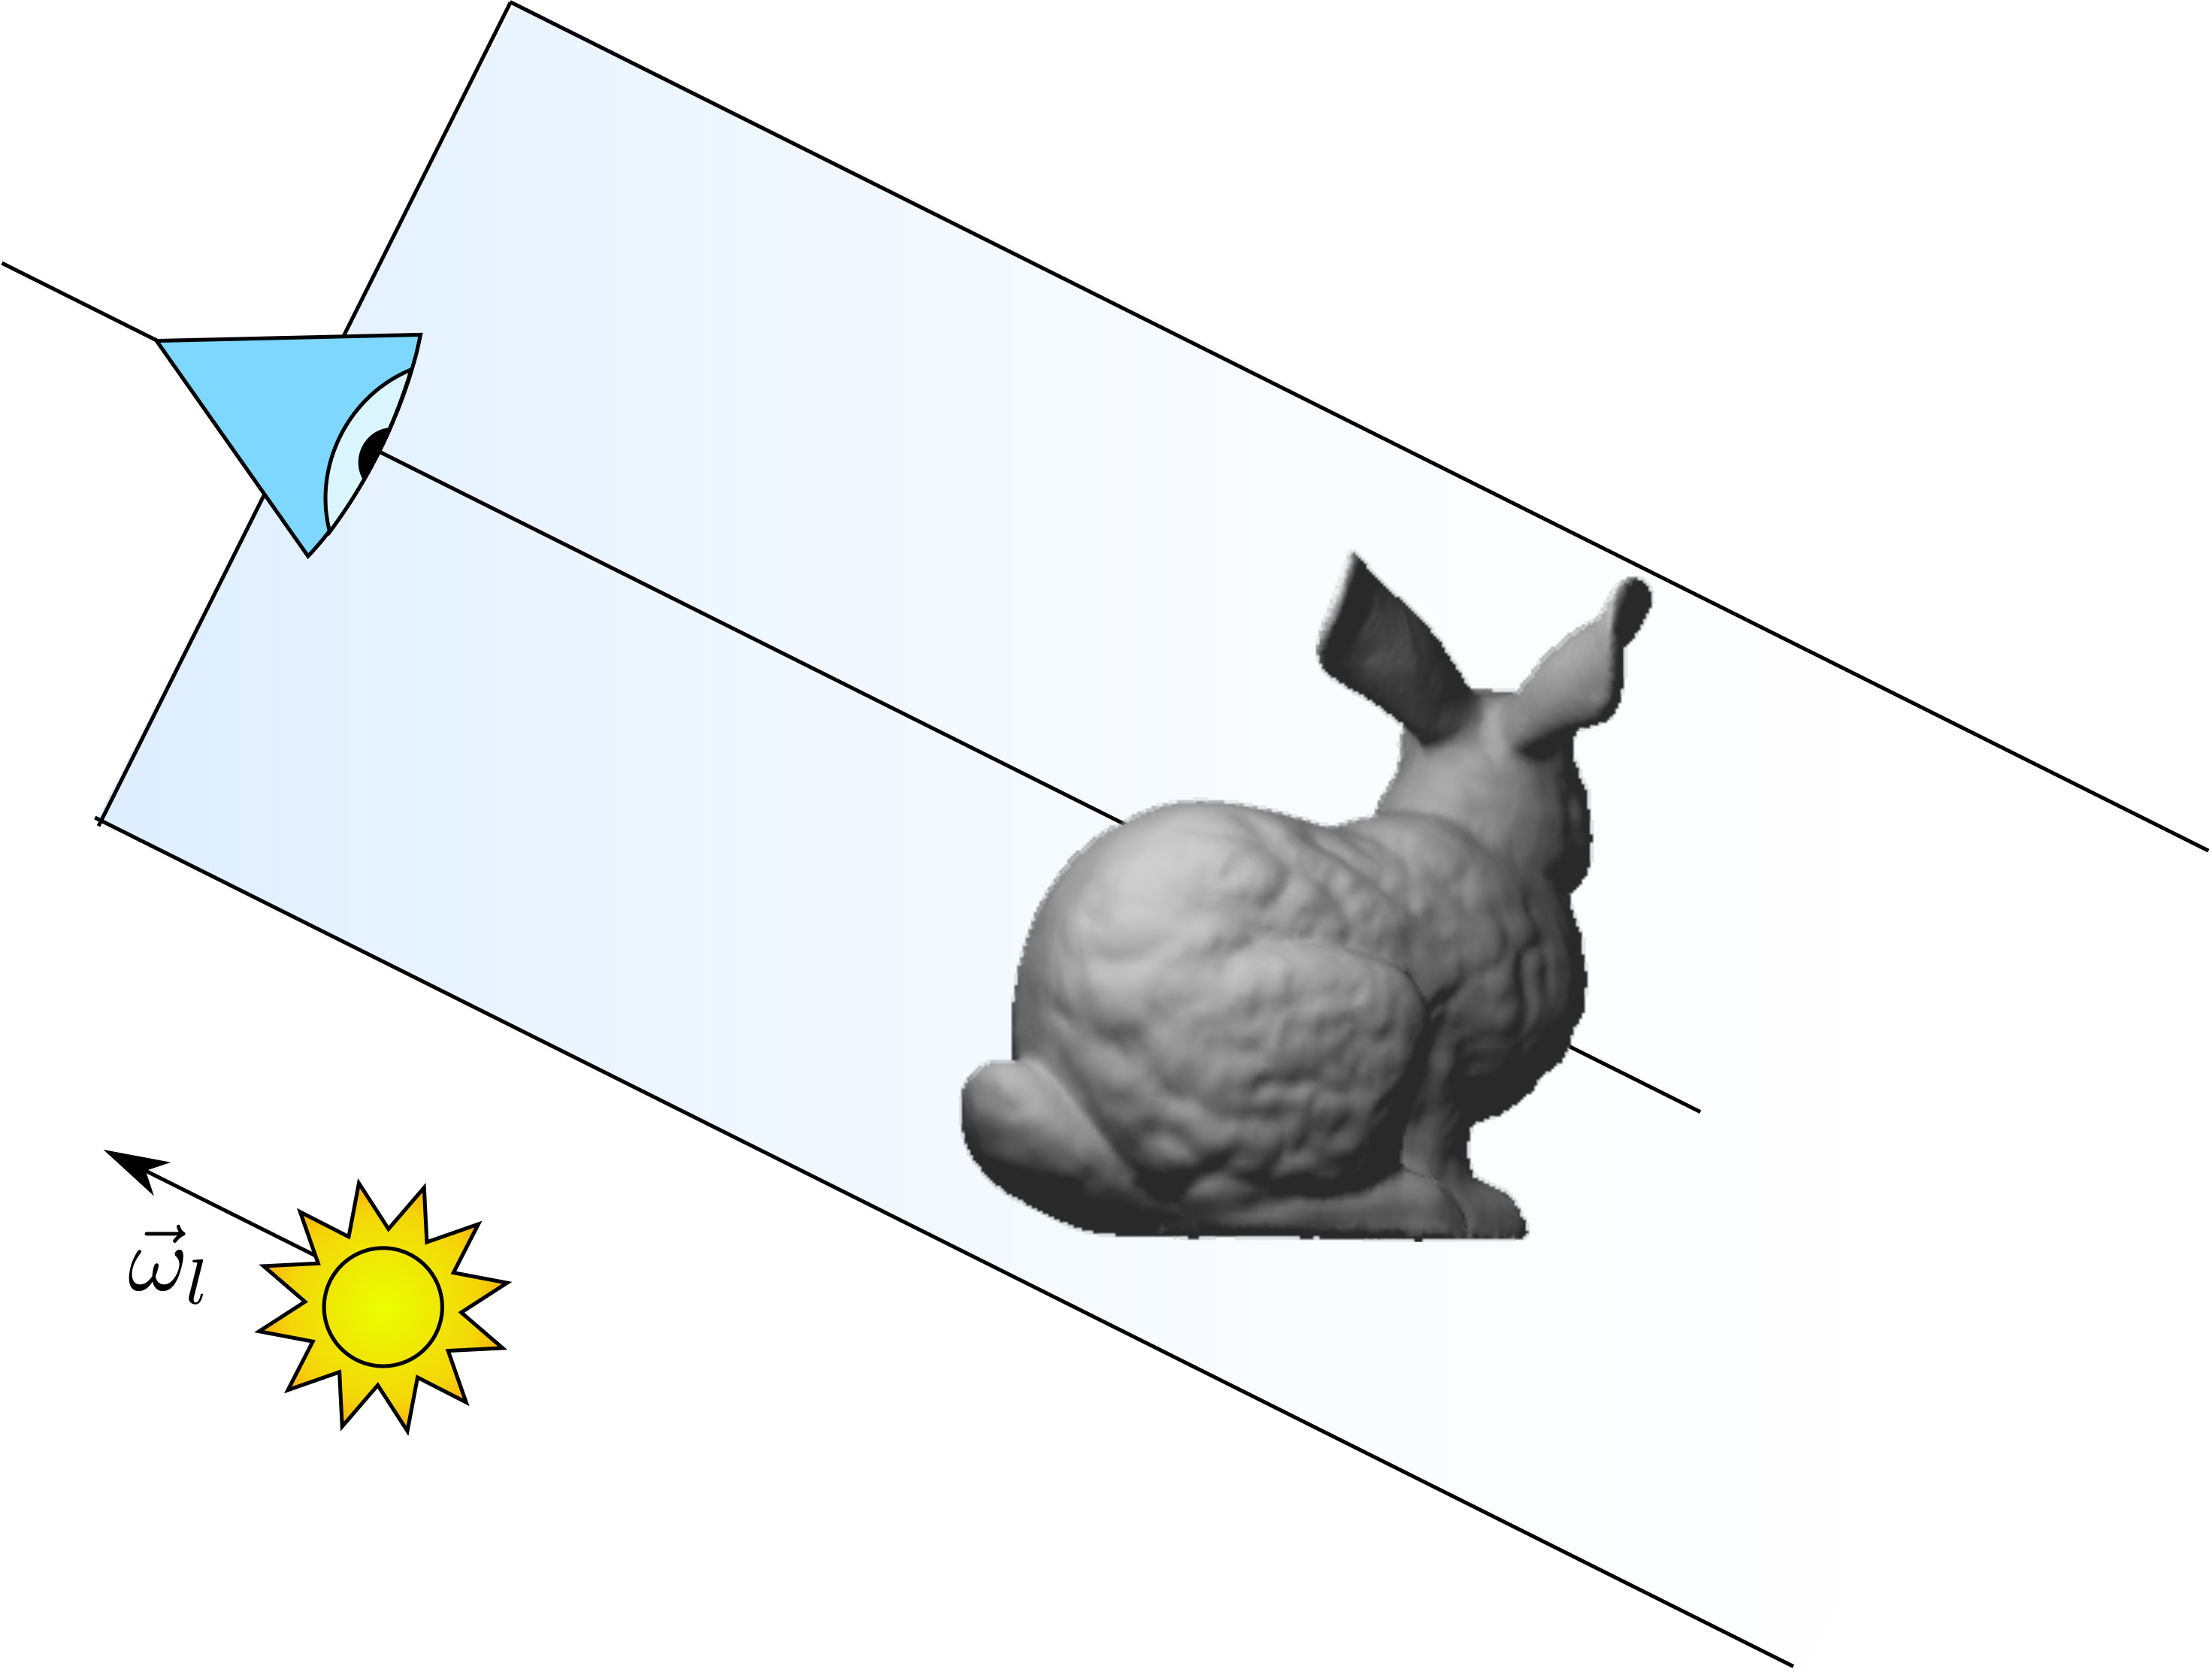
\includegraphics[width=0.3\textwidth]{step1.jpg} \hspace{0.5cm}	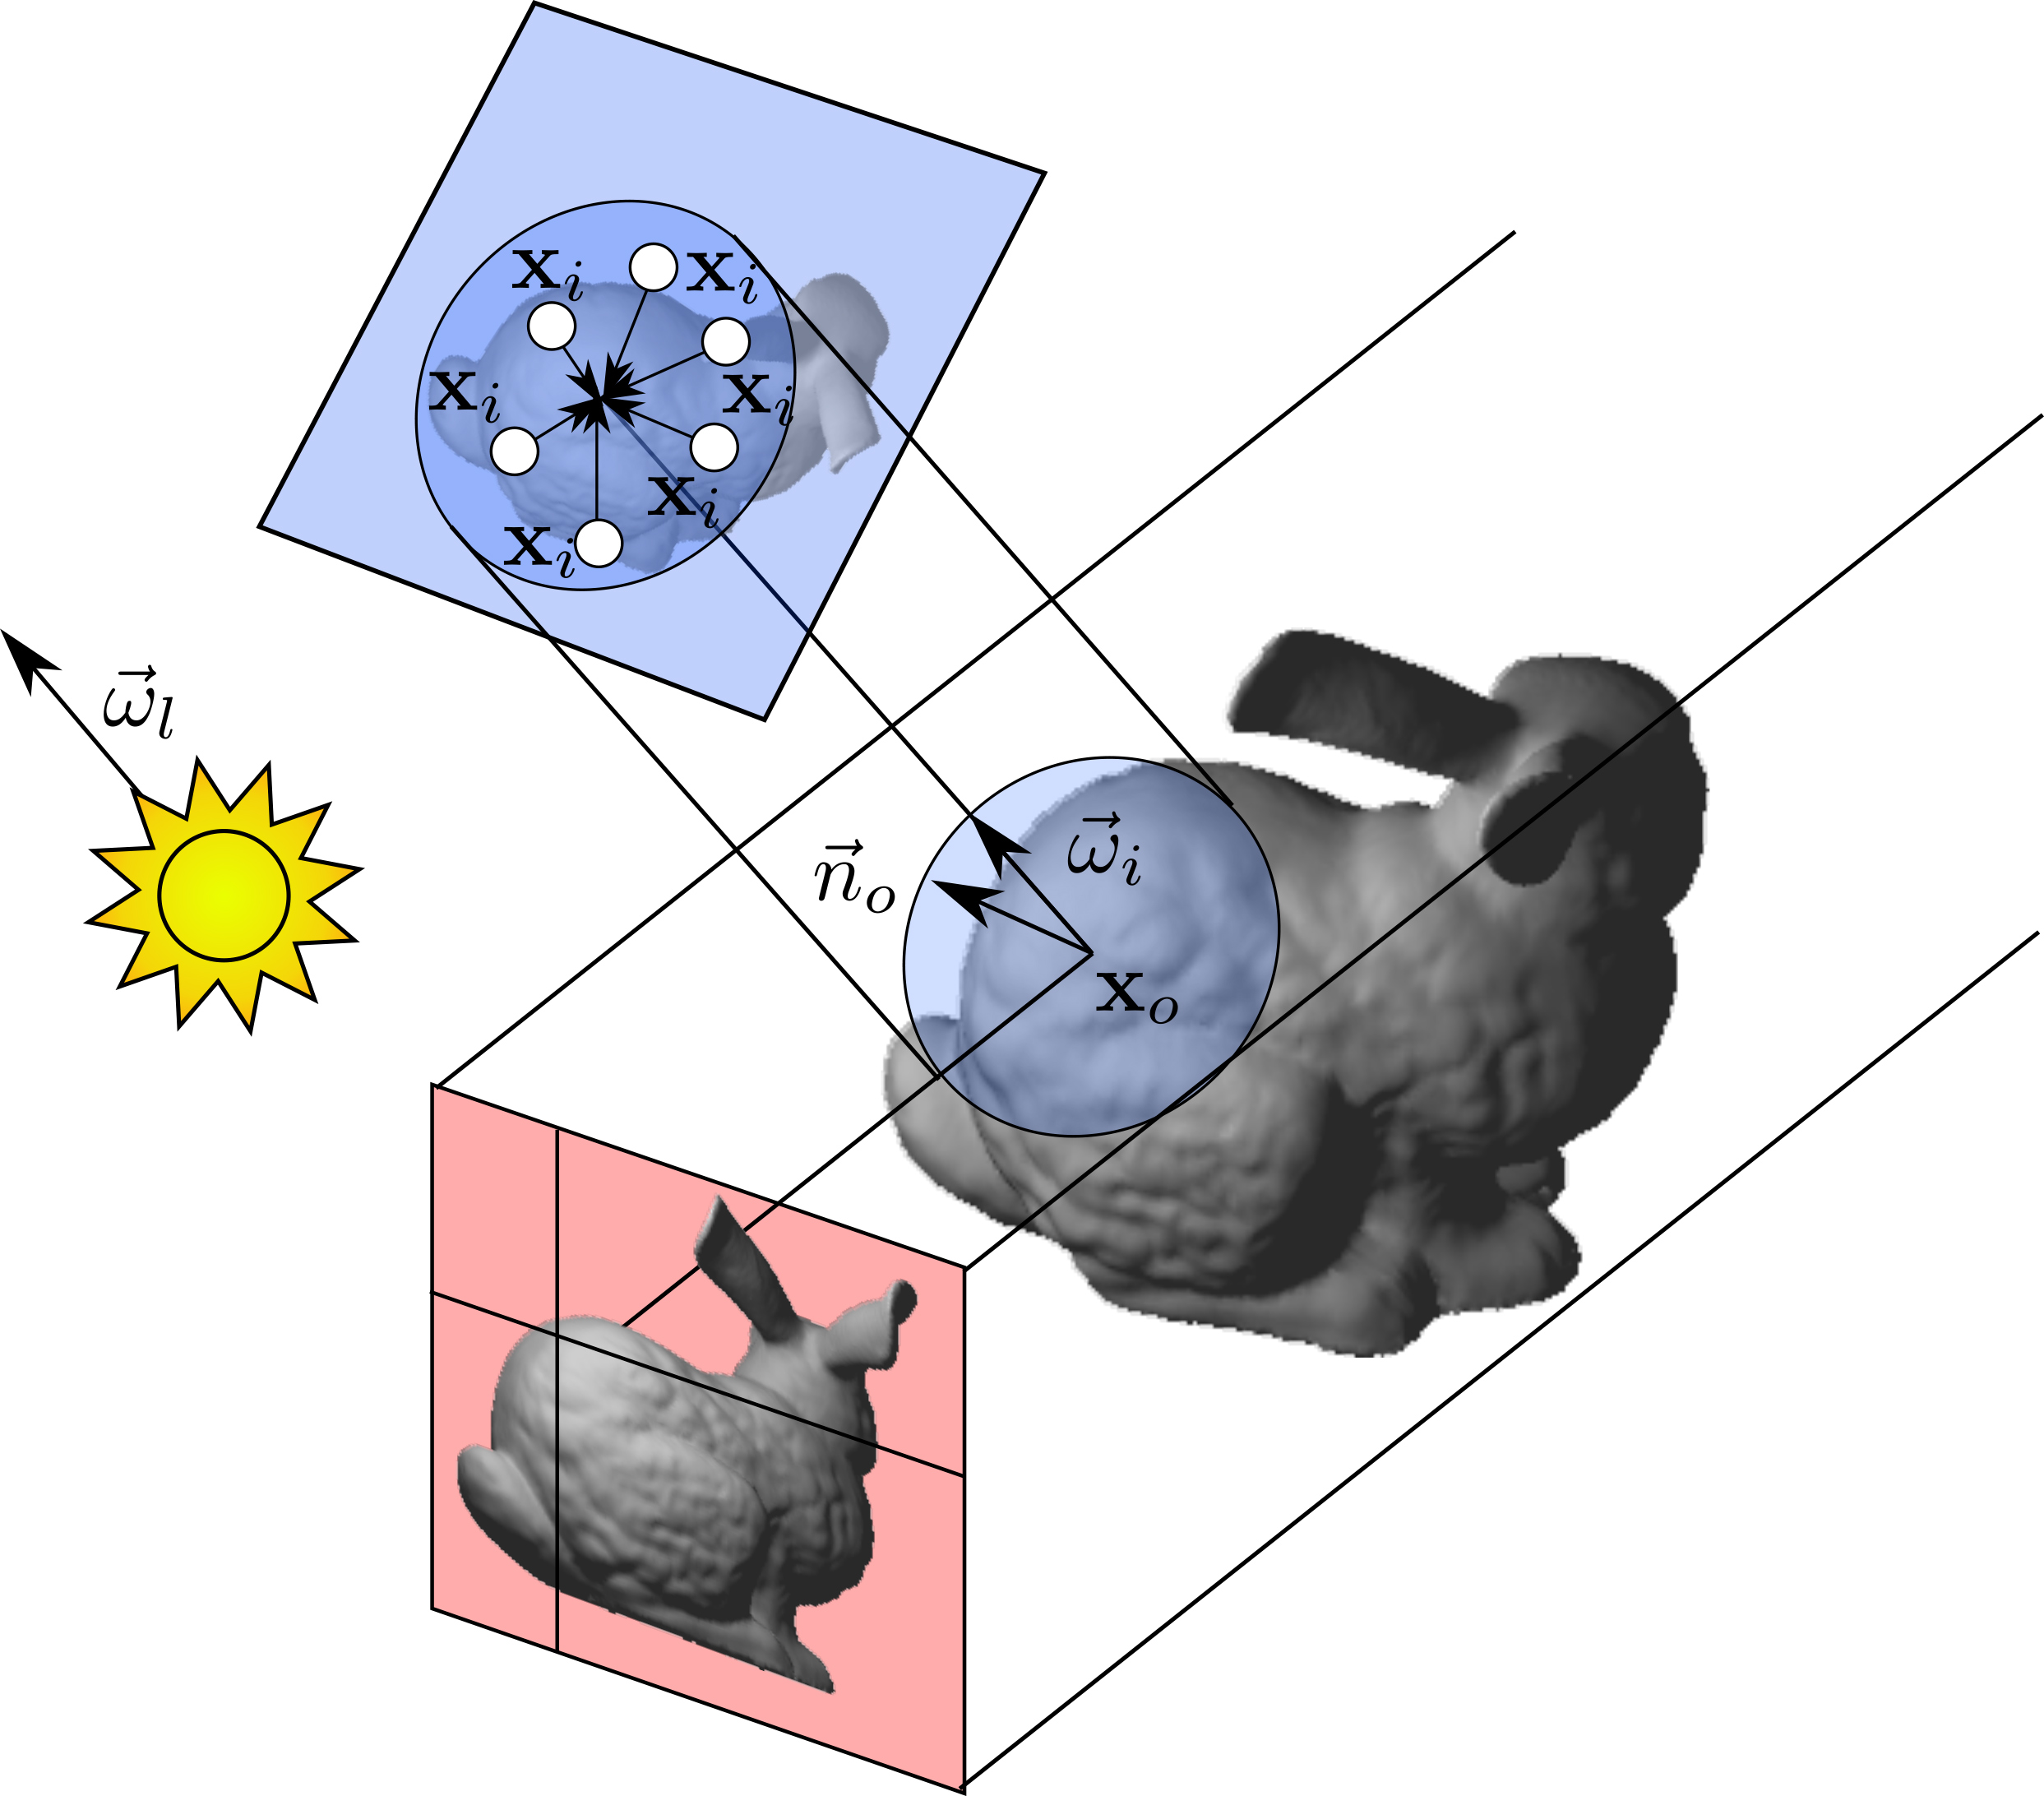
\includegraphics[width=0.3\textwidth]{step2.jpg} \hspace{0.5cm}	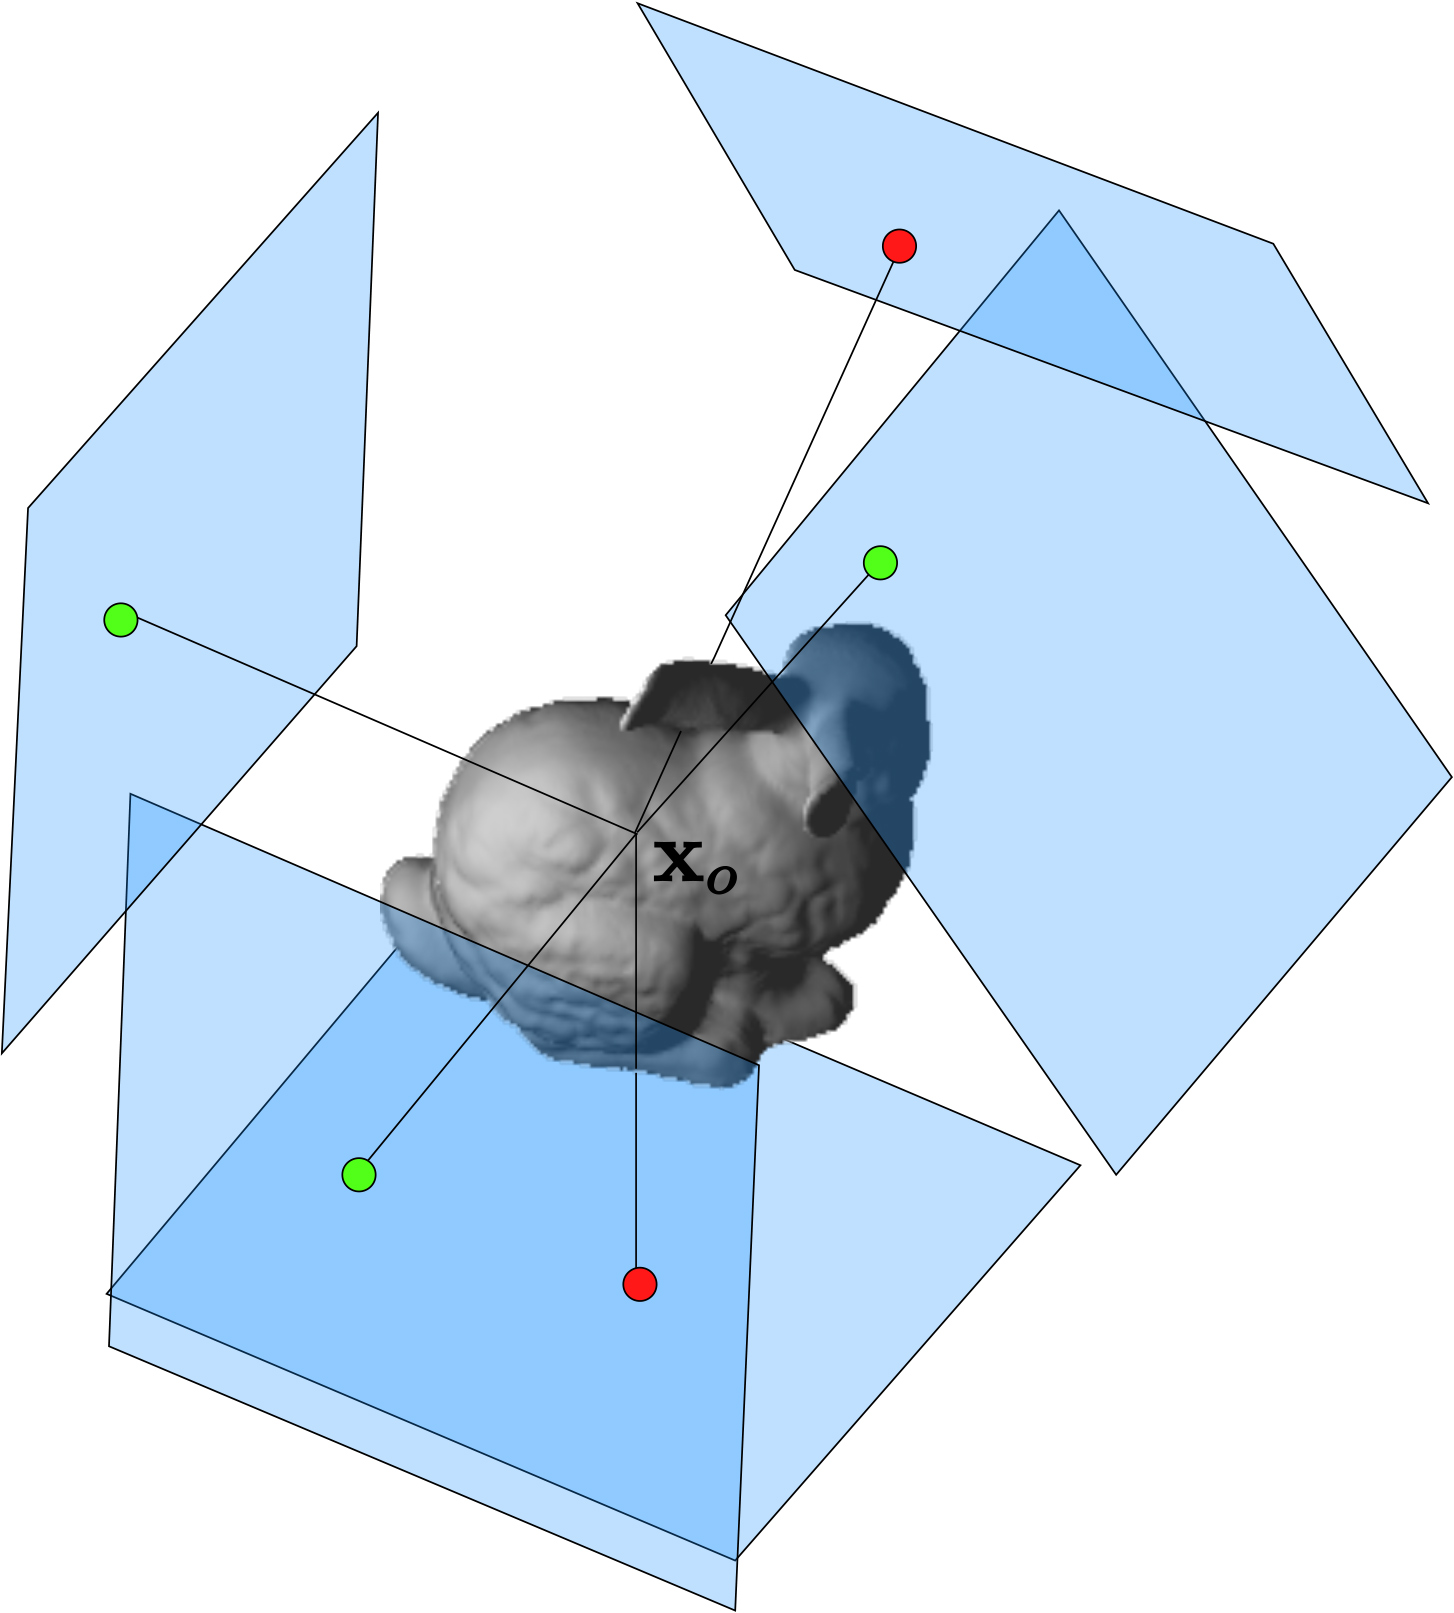
\includegraphics[width=0.25\textwidth]{step3.jpg}

\end{frame}

\begin{frame}
    \frametitle{Risultati (qualità)}
\begin{figure}
\vspace{0.3cm}
\centering
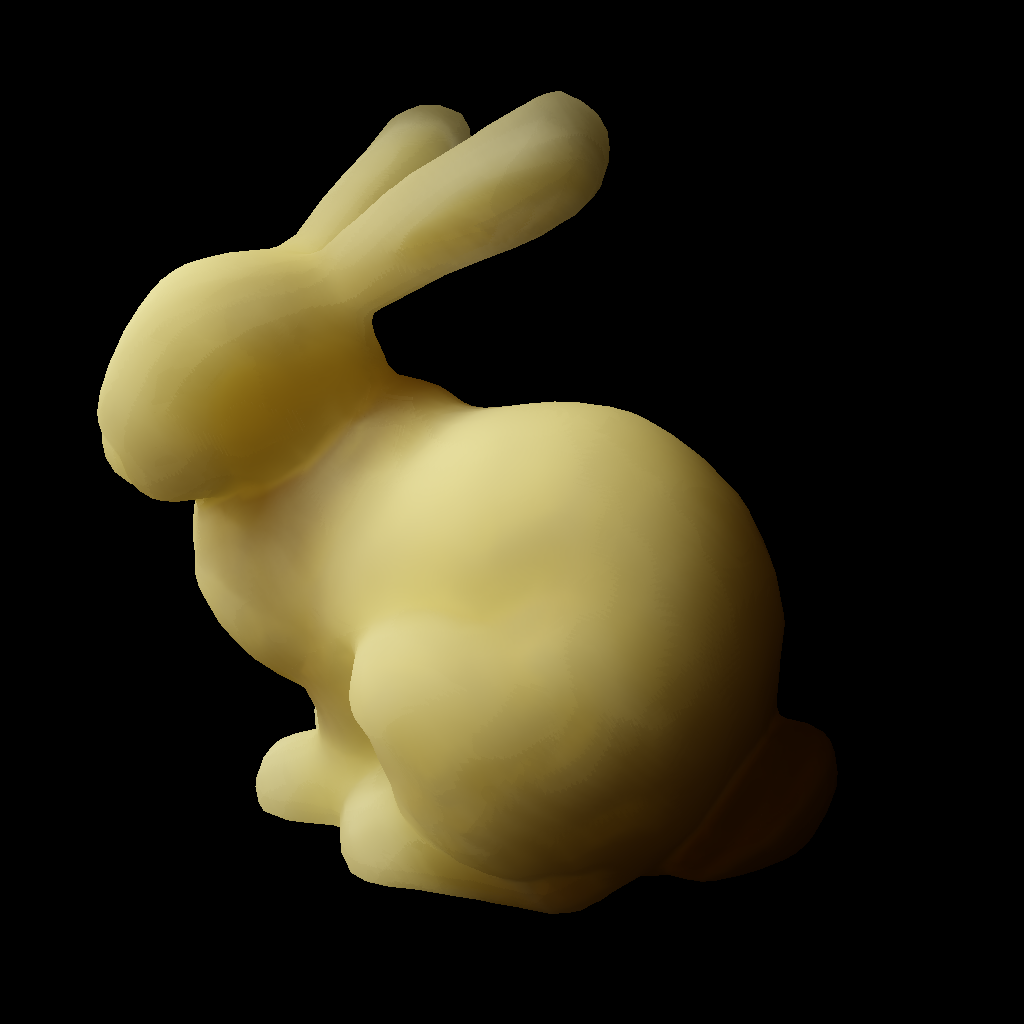
\includegraphics[width=0.55 \textwidth]{bunny}
\vspace{-0.3cm}
\caption{Stanford Bunny, parametri per patata. Si notino le ombre naturalmente generate dall'algoritmo.}
\end{figure}
\end{frame}

\begin{frame}
    \frametitle{Risultati (qualità)}
		\begin{figure}
\centering
\subfloat[{$\ N = 100$}]{
  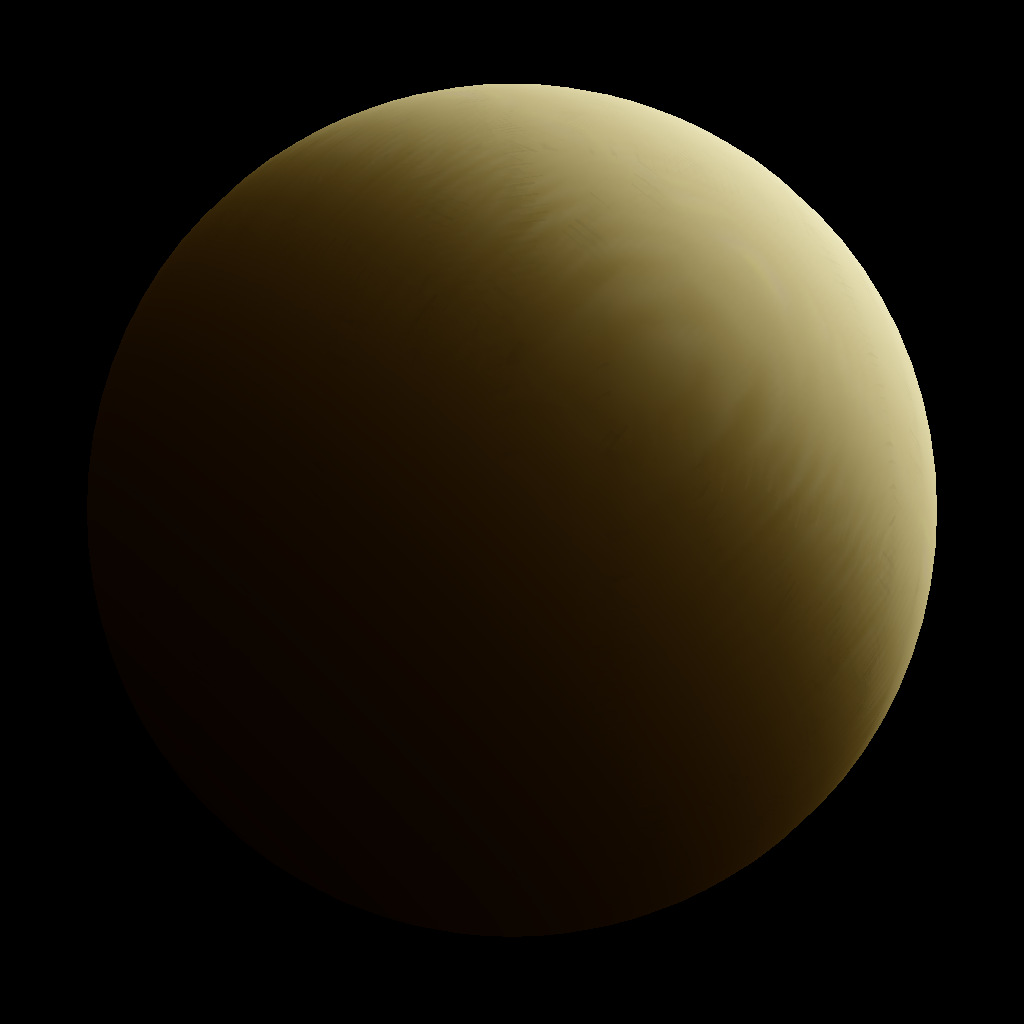
\includegraphics[width=0.25 \textwidth]{p100}
}
\subfloat[{$\ N = 1000$}]{
  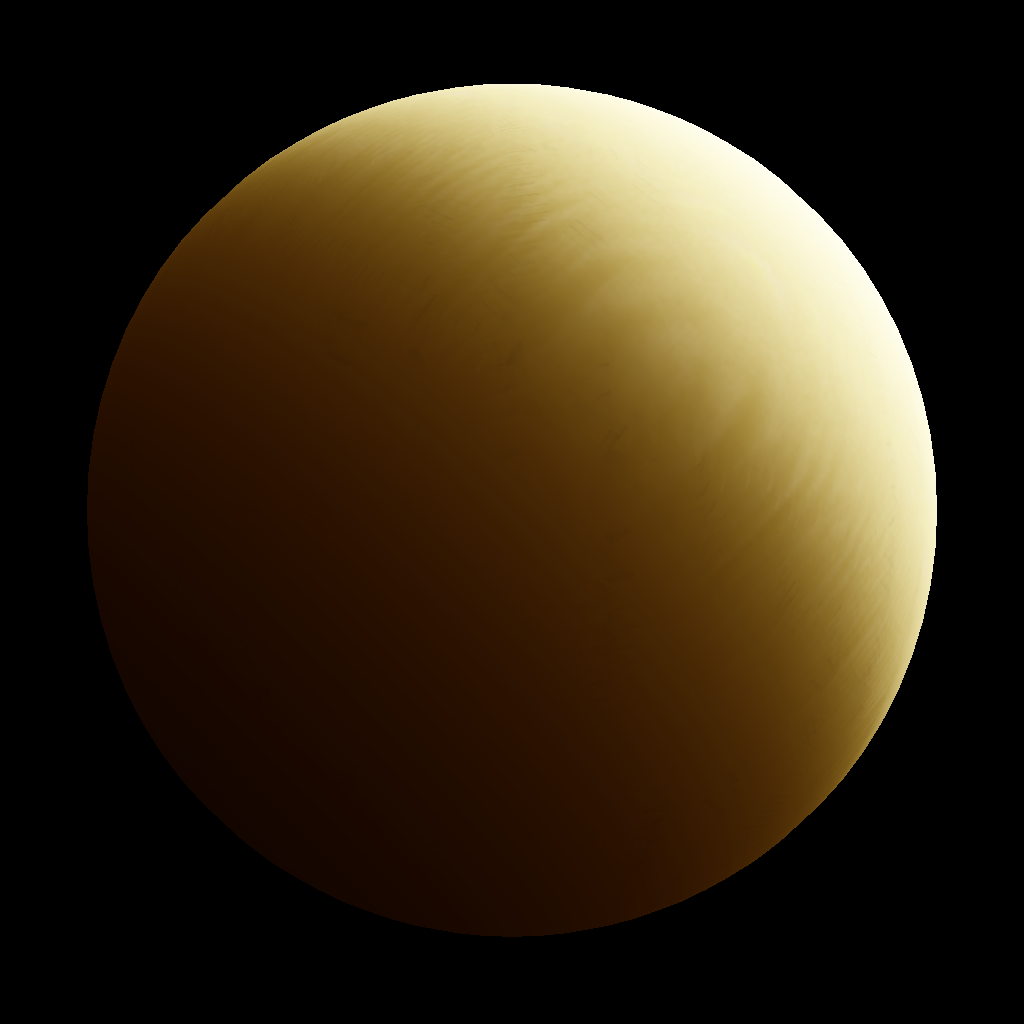
\includegraphics[width=0.25 \textwidth]{p1000}
}
\subfloat[$\ $Riferimento]{
  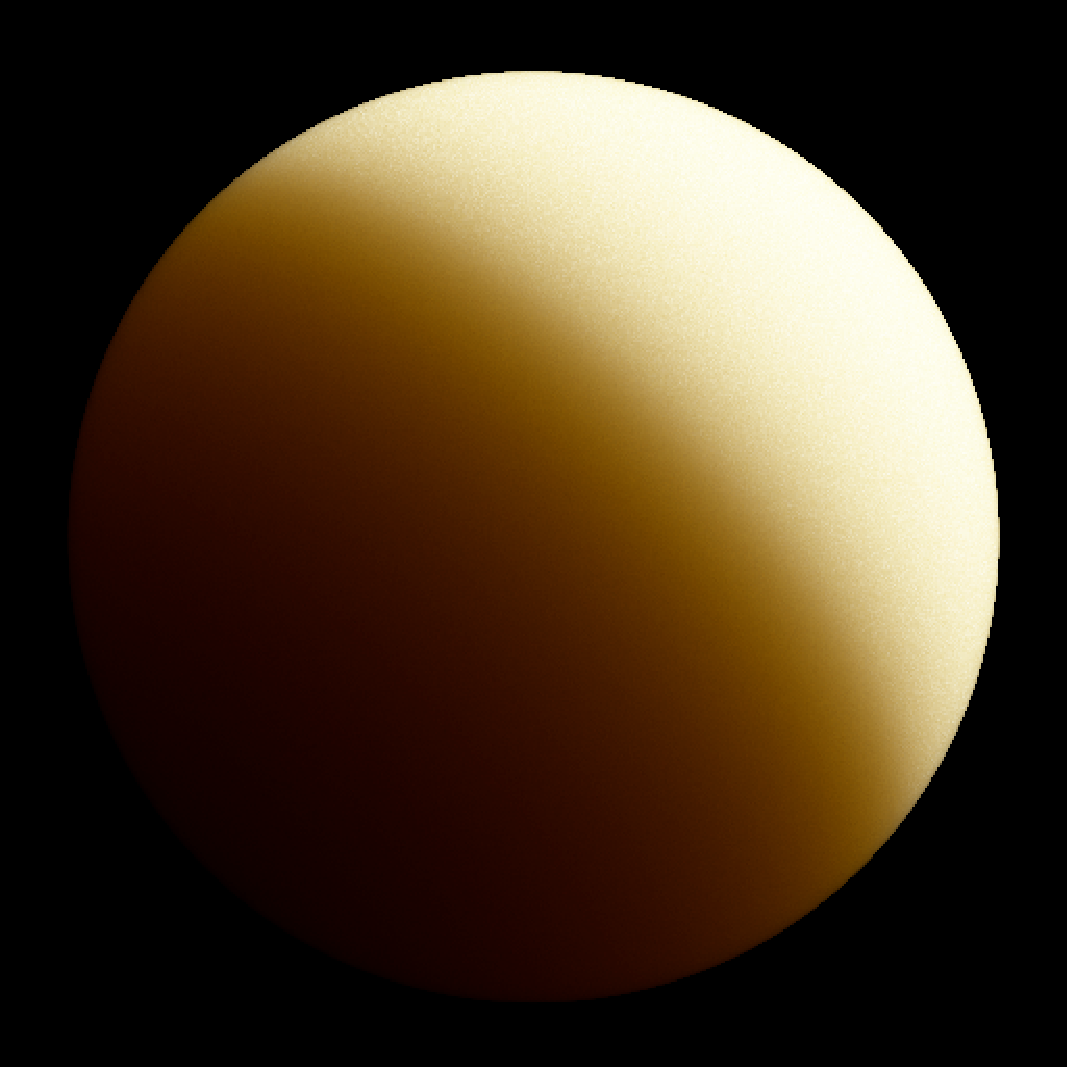
\includegraphics[width=0.25 \textwidth]{p}
} \\
\vspace{-0.4cm}
\subfloat[{$\ N = 100$}]{
  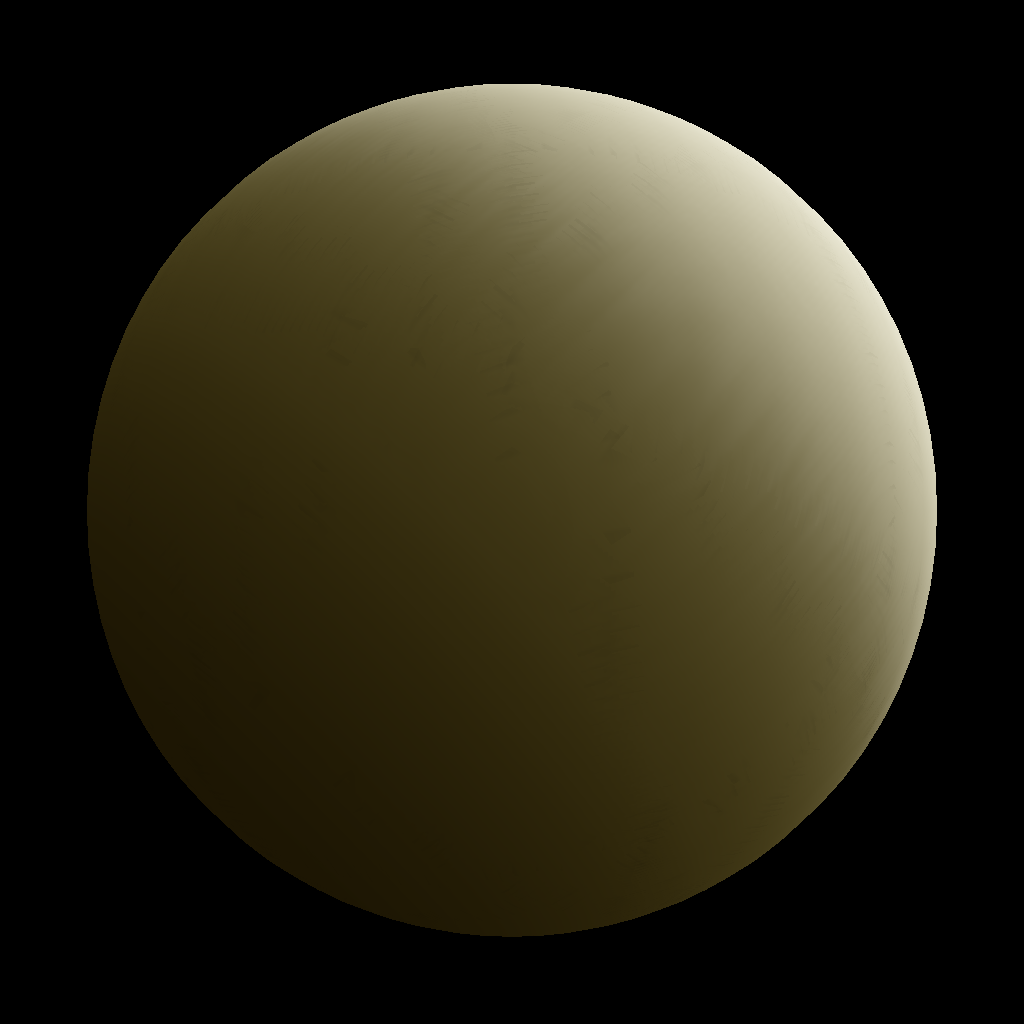
\includegraphics[width=0.25 \textwidth]{gj100}
} 
\subfloat[{$\ N = 1000$}]{
  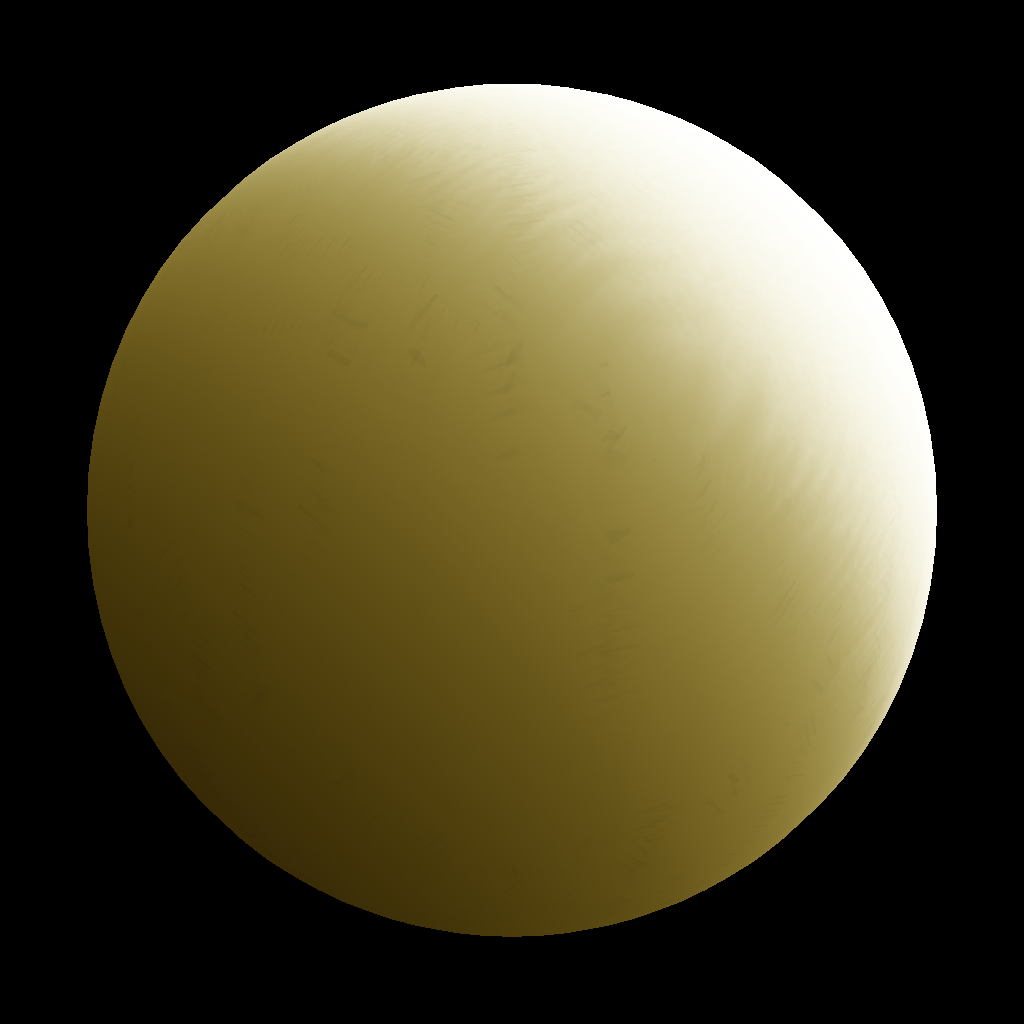
\includegraphics[width=0.25 \textwidth]{gj1000}
} 
\subfloat[$\ $Riferimento]{
  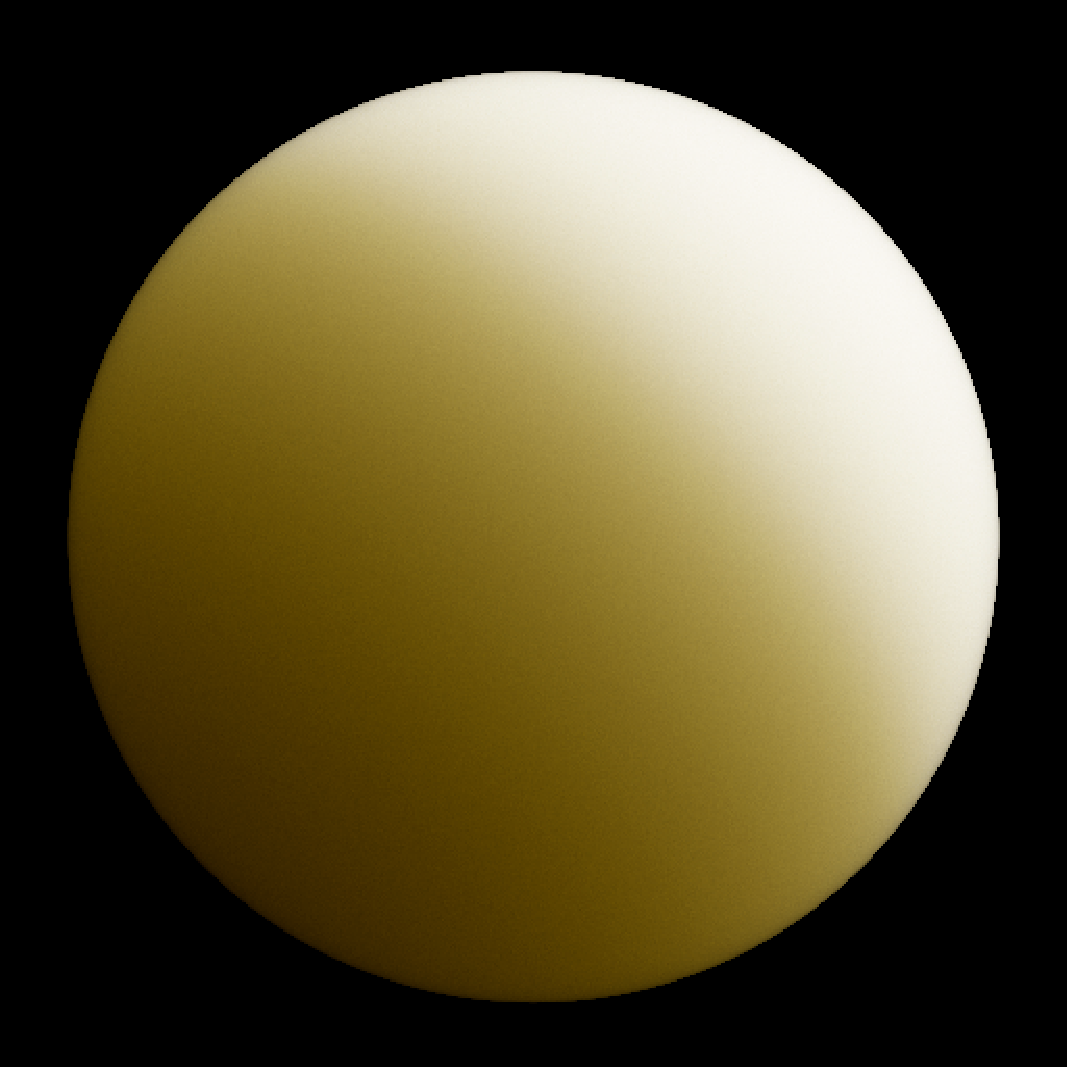
\includegraphics[width=0.25 \textwidth]{gj}
} 
\vspace{-0.2cm}
\caption{Comparazione dei risultati per patata e succo d'uva.}
\end{figure}

\end{frame}



\begin{frame}
    \frametitle{Risultati (qualità)}
				\begin{figure}
\centering
\subfloat[{$\ N = 50$ (ca. 90 millisecondi)}]{
  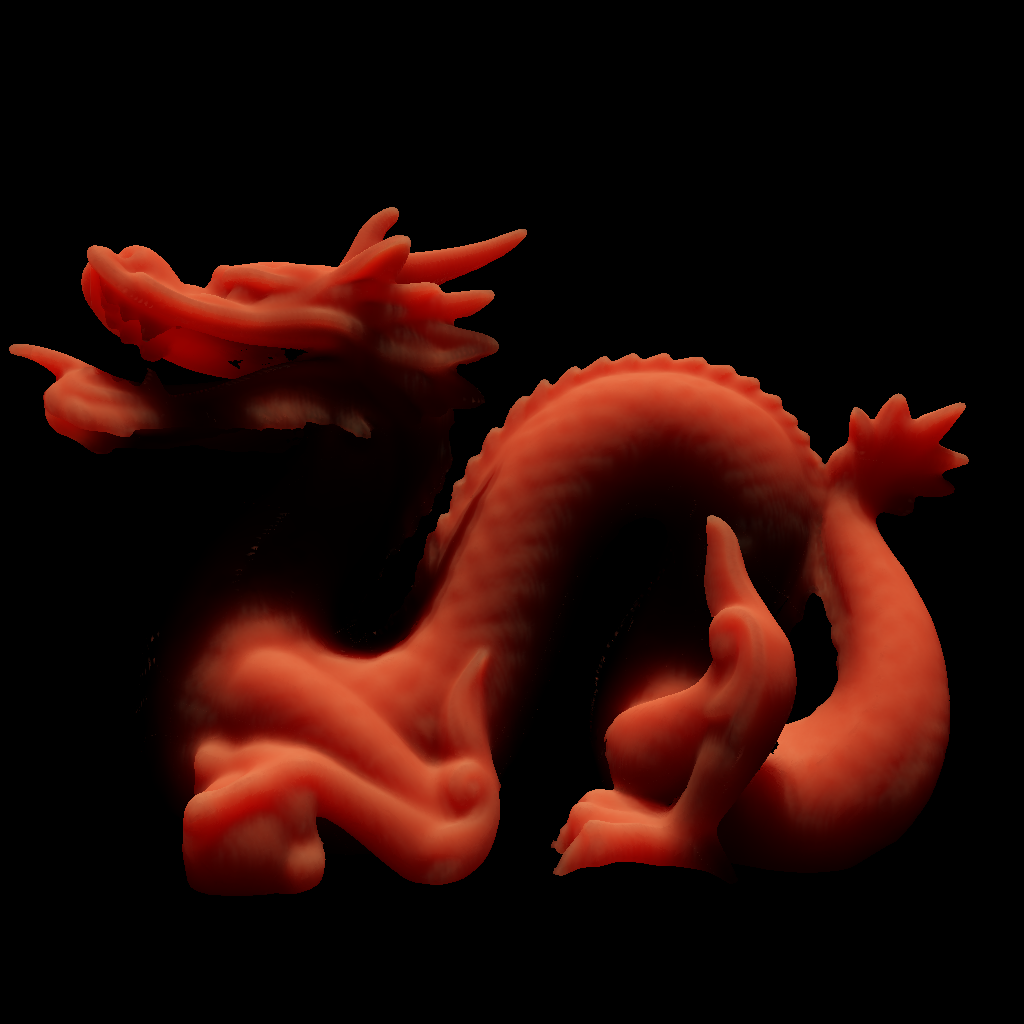
\includegraphics[width=0.45 \textwidth]{d50}
}
\subfloat[$\ $Riferimento (6 ore, 16 milioni di samples)]{
  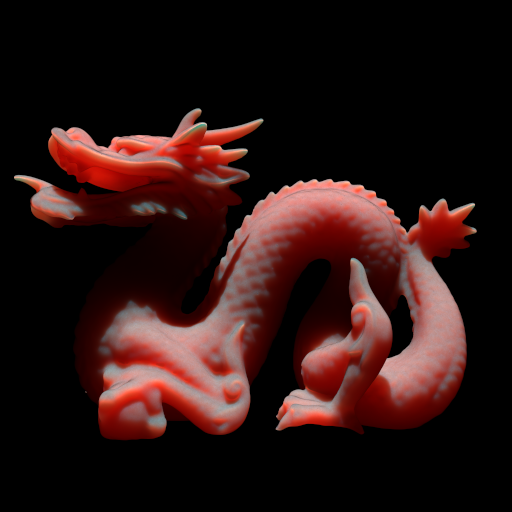
\includegraphics[width=0.45 \textwidth]{d}
} 
\vspace{-0.2cm}
\caption{Comparazione dei risultati per Stanford Dragon. Parametri per ketchup.}
\end{figure}

\end{frame}

\begin{frame}
    \frametitle{Risultati (performance)}
\renewcommand{\arraystretch}{1.8}
\begin{table}[!ht]
\centering
\begin{tabular}{p{3cm}l|l|l|l|l|}
\cline{3-6}
                             &      & \multicolumn{4}{c|}{Numero di samples ($N$)}                                          \\ \cline{3-6} 
Modello                        & \#$\Delta$& \multicolumn{1}{c|}{1} & \multicolumn{1}{c|}{10} & \multicolumn{1}{c|}{50} & \multicolumn{1}{c|}{100} \\ \hline
\multicolumn{1}{|l|}{Bunny}  & $10^4$ & \mycolor{2}.1                  & \mycolor{5}.3                 & \mycolor{19}.8                  & \mycolor{38}.2                 \\ \hline
\multicolumn{1}{|l|}{Dragon} & $10^5$ & \mycolor{12}.5                 & \mycolor{35}.2                  & \mycolor{140}.6                & \mycolor{275}.3                \\ \hline
\multicolumn{1}{|l|}{Buddha} & $10^6$ & \mycolor{96}.7                 & \mycolor{97}.7                  & \mycolor{128}.0                & \mycolor{216}.0                 \\ \hline
\end{tabular}
\caption{Timings in milliseconds of our method for different models and number of samples $N$ (potato material properties). One directional light, 16 directions for rendering and reconstructing.}
\end{table}
\end{frame}

\begin{frame}
    \frametitle{Conclusioni}

\begin{itemize}
	\item Abbiamo implementato una soluzione per il rendering veloce di materiali traslucidi usando BSSRDF direzionali
	\item Abbiamo ottenuto qualità paragonabili al path tracing
	\item Abbiamo ottenuto un miglioramento di 5 ordini di grandezza (millisecondi contro minuti/ore) 
	\item Abbiamo ottenuto un metodo flessibile e applicabile a engine professionali esistenti
\end{itemize}

\end{frame}


\end{document}
